% -----------------------------------------------
% Template for SMC 2016
% adapted from the template for SMC 2012 and 2011, which were adapted from that of SMC 2010
% -----------------------------------------------

\documentclass{article}
\usepackage{smc2017}
\usepackage{times}
\usepackage{ifpdf}
\usepackage[english]{babel}
\usepackage{cite}

%%%%%%%%%%%%%%%%%%%%%%%% Some useful packages %%%%%%%%%%%%%%%%%%%%%%%%%%%%%%%
%%%%%%%%%%%%%%%%%%%%%%%% See related documentation %%%%%%%%%%%%%%%%%%%%%%%%%%
%\usepackage{amsmath} % popular packages from Am. Math. Soc. Please use the 
%\usepackage{amssymb} % related math environments (split, subequation, cases,
%\usepackage{amsfonts}% multline, etc.)
%\usepackage{bm}      % Bold Math package, defines the command \bf{}
%\usepackage{paralist}% extended list environments
%%subfig.sty is the modern replacement for subfigure.sty. However, subfig.sty 
%%requires and automatically loads caption.sty which overrides class handling 
%%of captions. To prevent this problem, preload caption.sty with caption=false 
%\usepackage[caption=false]{caption}
%\usepackage[font=footnotesize]{subfig}


%user defined variables
\def\papertitle{\textit{Live Orchestral Piano}, a system for real-time orchestral music generation}
\def\firstauthor{L\'eopold Crestel}
\def\secondauthor{Philippe Esling}
\def\thirdauthor{Third author}

% adds the automatic
% Saves a lot of ouptut space in PDF... after conversion with the distiller
% Delete if you cannot get PS fonts working on your system.

\usepackage[pdftex,
pdftitle={\papertitle},
pdfauthor={\firstauthor, \secondauthor, \thirdauthor},
bookmarksnumbered, % use section numbers with bookmarks
pdfstartview=XYZ % start with zoom=100% instead of full screen; 
                 % especially useful if working with a big screen :-)
]{hyperref}
%\pdfcompresslevel=9

\usepackage[pdftex]{graphicx}
% declare the path(s) where your graphic files are and their extensions so 
%you won't have to specify these with every instance of \includegraphics
\graphicspath{{../Figures/}}
\DeclareGraphicsExtensions{.pdf,.jpeg,.png}

\usepackage[figure,table]{hypcap}



% % % % % % % % % % %
% % % % % % % % % % %
% % % % % % % % % % %

\usepackage{amsmath,amssymb} % For including math equations, theorems, symbols, etc
\usepackage{bm}
\usepackage{graphicx} % Required for including images
\graphicspath{{../Figures/}} % Set the default folder for images
% Makecell 
\usepackage{makecell}
\renewcommand\theadalign{cb}
\renewcommand\theadfont{\bfseries}
\renewcommand\theadgape{\Gape[4pt]}
\renewcommand\cellgape{\Gape[4pt]}

% % % % % % % % % % %
% % % % % % % % % % %
% % % % % % % % % % %



%setup the hyperref package - make the links black without a surrounding frame
\hypersetup{
    colorlinks,%
    citecolor=black,%
    filecolor=black,%
    linkcolor=black,%
    urlcolor=black
}


% Title.
% ------
\title{\papertitle}

%Two addresses
%--------------
 \twoauthors
   {\firstauthor} {IRCAM \\ %
     {\tt \href{mailto:leopold.crestel@ircam.fr}{leopold.crestel@ircam.fr}}}
   {\secondauthor} {IRCAM \\ %
     {\tt \href{mailto:philippe.esling@ircam.fr}{philippe.esling@ircam.fr}}}


% ***************************************** the document starts here ***************
\begin{document}
%
\capstartfalse
\maketitle
\capstarttrue
%
\begin{abstract}
This paper introduces the first system for performing automatic \textit{orchestration} based on a real-time piano input. We believe that it is possible to learn the underlying regularities existing between piano scores and their orchestrations by notorious composers, in order to automatically perform this task on novel piano inputs. To that end, we investigate a class of statistical inference models based on the \textit{Restricted Boltzmann Machine} (\textit{RBM}). We introduce a specific evaluation framework for orchestral generation based on a prediction task in order to assess the quality of different models. As prediction and creation are two widely different endeavours, we discuss the potential biases in evaluating temporal generative models through prediction tasks and their impact on a creative system. Finally, we introduce an implementation of the proposed models called \textit{Live Orchestral Piano} (LOP), which allows to perform real-time projective orchestration of a MIDI keyboard input.
Generated orchestration generated by the different models we investigated can be found at this address \url{https://qsdfo.github.io/LOP/}.
\end{abstract}
%

\section{Introduction}
% Orchestration classique
%% Musical orchestration : why is it so hard ?
% Orchestration
\textit{Orchestration} is the subtle art of writing musical pieces for the orchestra, by combining the properties of various instruments in order to achieve a particular sonic rendering \cite{koechli_orch,Rimsky-Korsakov:1873aa}. Because it extensively relies on spectral characteristics, orchestration is often referred to as the art of manipulating instrumental timbres \cite{mcadams2013timbre}. Timbre is defined as the property which allows listeners to distinguish two sounds produced at the same pitch and intensity.
% -> Timbre
Hence, the sonic palette offered by the pitch range and intensities of each instrument is augmented by the wide range of expressive timbres produced through the use of the different playing styles.
% Non linear spectral behaviours
Furthermore, it has been shown that some instrumental mixtures can not be characterized by a simple summation of their spectral components, but can lead to a unique \textit{emerging timbre}, with phenomenon such as orchestral blend \cite{tardieu2012perception}.
% -> Combinatoire
Given the number of different instruments in a symphonic orchestra, their respective range of expressiveness (timbre, pitch and intensity), and the phenomenon of emerging timbre, one can foresee the extensive combinatorial complexity embedded in the process of orchestral composition.

\textbf{Those difficulties have been a major obstacle towards the construction of a scientific basis for the study of orchestration. From a mathematical point of view, it seems that no set of descriptors can exhaustively fit with the perceptual complexity of timbre \cite{peeters2011timbre}. From a musical point of view, there is a lack of specific symbolic notation for timbre, and orchestration remains an empirical discipline taught through the observation of existing orchestration examples \cite{piston-orch}. //USELESS}

Among the different writing techniques for orchestral works, one of them consists in first writing an harmonic and rhythmic structure in the form of a piano score and then adding the timbre dimension by spreading the different voices over the various instruments \cite{piston-orch}. We refer to this operation of extending a piano draft to an orchestral score as \textit{projective orchestration} \cite{eslingthesis}.
The orchestral repertoire contains a large number of examples of projective orchestration (such as the piano reductions by Liszt of Beethoven symphonies or the \textit{pictures at an exhibition}, a piano piece by Moussorgsky orchestrated by Ravel among several notorious composers). By observing a case of projective orchestration (see \ref{fig:orch}), we can clearly see that this process involves more than the mere allocation of notes written on the piano score across the different instruments. It rather implies harmonic enhancements and timbre manipulations to underline the already existing harmonic and rhythmic structure \cite{mcadams2013timbre}. However, the visible correlations between a piano score and its orchestrations appear as a fertile framework for laying the foundations of a computational exploration of orchestration.

\begin{figure}
\centering
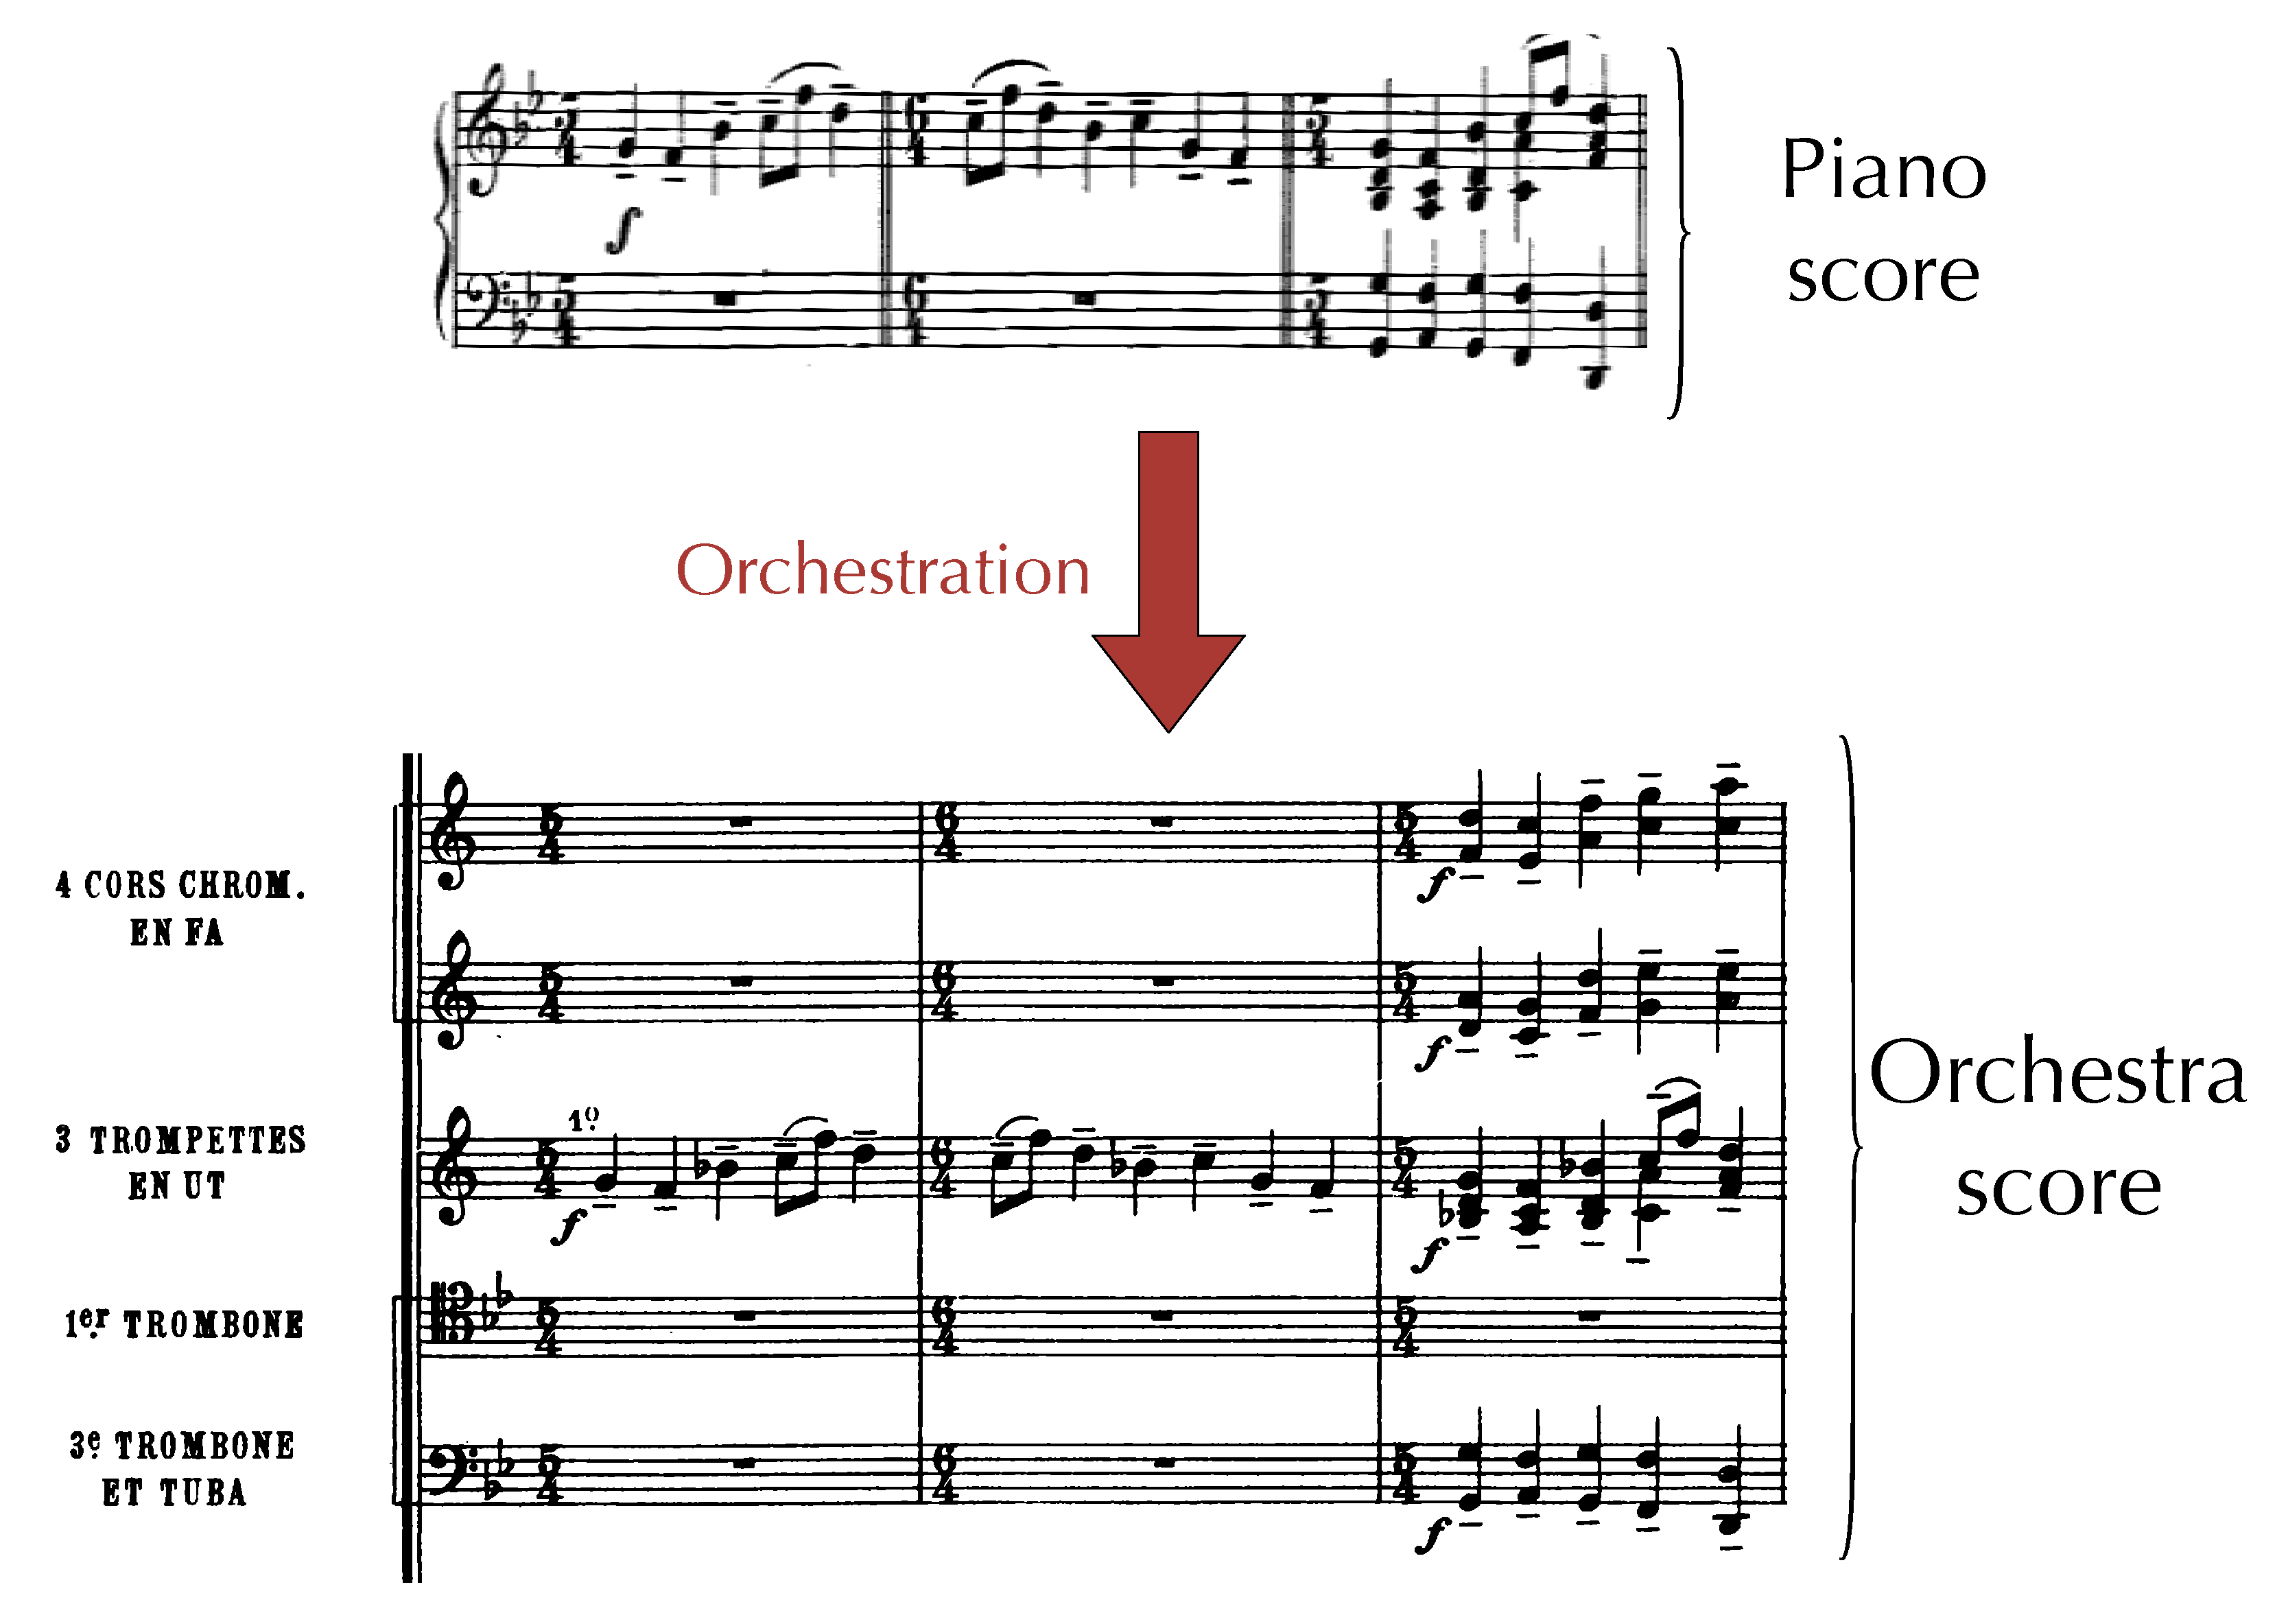
\includegraphics[scale=0.15]{Data_representation/orch}
\caption{\textit{Projective orchestration}. A piano score is projected on an orchestra. Even though a wide range of orchestrations exist for a given piano score, all of them will share strong relations with the original piano score. One given orchestration implicitly embeds the knowledge of the composer about timbre and orchestration.}
\label{fig:orch}
\end{figure}

Statistical inference covers a range of methods aimed at automatically extracting a structure from observations. These approaches hypothesize that a particular type of data might be structured by an underlying probability distribution. The objective is to deduce properties of this distribution, by observing a set of those data. 
If the structure of the data is efficiently extracted and organized, it should be possible in turn to generate novel examples.
%Thus, our objective is to build a system of automatic projective orchestration. 
We believe that learning the underlying distribution of a corpus of piano scores and their orchestrations by famous composers through statistical inference is a promising lead toward the automatic generation of orchestrations with a sensible timbre structure.
In the context of projective orchestration, the data are defined as the scores, formed by a series of pitches and intensities for each instrument. The set of observations is a set of projective orchestrations performed by famous composers, and the probability distribution would model the set of notes played by each instrument conditionally on the corresponding piano score.

It might be surprising at first to rely solely on symbolic information (scores) whereas we insisted on the fact that orchestration is the art of timbre, typically not represented in the musical notation but rather conveyed in the signal information (audio recording).
However, we make the assumption that spectrally consistent orchestrations could be generated from a purely symbolic learning by uncovering the composers' knowledge about timbre embedded in the score. As we rely on the works of composers that effectively took into account the subtleties of timbral effects, these symbolic relationships embed the spectral information.

A wide range of statistical inference models have been devised, among which deep learning recently appeared as a  promising field in artificial intelligence and representation learning \cite{bengio2013representation,LeCun:2015aa}.
Deep learning techniques have already been successfully applied to several musical applications and neural networks are now the state of the art in most music information retrieval tasks \cite{humphrey2012moving,lee2011unsupervised,boulanger2013audio} and for speech recognition and synthesis \cite{hinton2012deep,DBLP:journals/corr/OordDZSVGKSK16}. Generative systems working with symbolic information (musical scores) also appeared as a prosperous framework for deep learning models. Successful applications have been made to automatic music composition \cite{eck2002finding,lavrenko2003polyphonic,bosley2010learning,boulanger2012modeling,Johnson2015}
automatic harmonization \cite{Sun} and style transfer \cite{Pachet2016}. However, the automatic projective orchestration task has never been investigated using deep learning methods and this paper is the first attempt to do so.

The final objective of the model we are trying to build is to generate orchestrations from unseen piano scores.
We propose in this article to investigate a class of models called \textit{Conditional RBM} \cite{taylor2006modeling}. Conditional models implement a dependency mechanism that seems adapted to model the influence of the piano score over the orchestral score.

In order to rank the different models, it is important to devise a quantitative evaluation framework. Designing a criterion assessing the performance of a generative model is a major difficulty for creative systems. In the polyphonic music generation field, a predictive task is commonly used \cite{boulanger2012modeling,lavrenko2003polyphonic,DBLP:journals/corr/YaoCVDD15}. Relying on these works, we introduce a specific framework for projective orchestration and made a benchmark of the introduced models in this framework. We then propose a qualitative analysis of both the models and the evaluation framework to explain the results obtained.

Finally, using the defined performance criterion we selected the most efficient model and implemented it in a system called \textit{Live Orchestral Piano} (LOP), an interface for real-time orchestration from a piano input.

The remainder of this paper is organized as follows. The first section introduces the state of the art in conditional models, in which RBM, cRBM and \textit{FGcRBM} models are detailed. The projective orchestration task is presented in the next section along with an evaluation framework based on a frame-level accuracy measure. The introduced models are evaluated within this framework and compared to existing models. Then, we introduce \textit{LOP}, the real-time projective orchestration system. Finaly, we provide our conclusions and directions of future work.

\section{State of the art}
In this section, three statistical inference models are detailed. The \textit{RBM}, \textit{cRBM} and \textit{FGcRBM} are presented by increasing level of complexity.
\subsection{Restricted Boltzmann Machine}
\subsubsection{An energy based model}
% Energy -> probability
The restricted Boltzmann Machine (\textit{RBM}) is a graphical probabilistic model. Stochastic binary-valued 
visible units $\bm{v} = \{ v_1, .., v_{n_v} \}$ and hidden units $\bm{h} = \{ h_1, .., h_{n_h} \}$ , where $n_h$ and $n_v$ is the number of hidden and visible unit, are tied together through the weights $\bm{W}$ by conditional probabilities
\begin{align}
\label{eq:conditional_rbm}
p(v_i=1|\bm{h}) = \sigma(a_i + \sum_{j=1}^{n_h} W_ij h_j)\\
p(h_j=1|\bm{v}) = \sigma(b_j + \sum_{j=1}^{n_h} W_ij h_j)
\end{align}
where $\sigma(x) = \frac{1}{1 + exp(-x)}$ is the sigmoid function

The joint probability of the visible and hidden variables is given by
\begin{equation}
p_{model}(\bm{v},\bm{h}) =  \frac{\exp^{-E(\bm{v},\bm{h})}}{Z}
\end{equation}
where
\begin{equation}
\label{eq:energy}
E(\bm{v},\bm{h}) = - \sum_{i=1}^{n_{v}} a_i v_{i}  - \sum_{i=1}^{n_v} \sum_{j=1}^{n_h} v_{i} W_{ij} h_{j} - \sum_{j = 1}^{n_h} b_j h_{j}
\end{equation}
with $\bm{\Theta} = \left\{\bm{W},\bm{b},\bm{a}\right\}$ the parameters of the network.

\subsubsection{Training procedure}
% A typical cost function = likelihood
The values of the parameters $\bm{\Theta}$ of a \textit{RBM} are tuned through the minimization of an error function.
A popular and well suited error function to train probabilistic models is the negative log-likelihood 
\begin{equation}
\label{eq:likelihood}
\mathcal{L(\bm{\theta}|\mathcal{D})}  = \frac{1}{N_{\mathcal{D}}} \sum_{\bm{v^{(l)}} \in \mathcal{D}} - \ln \left( p(\bm{v^{(l)}}|\bm{\theta})\right)
\end{equation}
where $\mathcal{D}$ is the training dataset and $N_{\mathcal{D}}$ the number of points it contains.

% Likelihood ? Intractable
Ideally, the training procedure consists in modifying the parameters $\Theta$ of the model along the gradient of the error function.
However, the gradient of the negative log-likelihood is intractable.
% Contrastive divergence
The contrastive divergence (\textit{CD}) algorithm \cite{Fischer2012,hinton2010practical} resort to an approximation of this quantity obtained through running a Gibbs sampling chain.
%DETAILS + SCHEMA
It consists in alternatively sampling from the visible and hidden units from the conditional probabilities defined in equations \ref{eq:conditional_rbm} in order to obtain a vector of visible units close to the real distribution of the model. The vector from the training set is often referred to as the positive sample, whereas the vector obtained at the end of the Gibbs chain is called negative sample.
\textit{CD} guarantees that the Kullback-Leibler divergence between the model and data distribution is reduced after each iteration\cite{hinton2002training}, and an acceptable approximation should be found after large number of \textit{CD} steps.

\subsection{Conditional models}
We introduce two conditional models that implement a notion of conditional dependency of the visible units given context units (denoted $\bm{x}$) :  the \textit{cRBM} and \textit{FGcRBM}. More details can be found in the original paper \cite{taylor2009factored}.

\subsubsection{Conditional RBM}
In the \textit{cRBM} model, the influence of the context units is implemented by an additive term on the bias of both visible and hidden units.
\begin{align}
\tilde{a}_i = a_i + \sum_{k=1}^{n_x} A_{ki} x_k\\
\tilde{b}_i = b_j + \sum_{k=1}^{n_x} B_{kj} x_k
\end{align}
$\tilde{\bm{a}}$ and $\tilde{\bm{b}}$ are called dynamic biases, by opposition to the static biases $\bm{a}$ and $\bm{b}$. The additive term is a linear combination of a third set of random variables called context units $\bm{x} = \{ x_1, .., x_k, .., x_{n_x} \}$.
Through matrices of parameters $\bm{A}$ and $\bm{B}$, the context units can stimulate or inhibit the hidden or visible units by translating the activation function along the input axis. After replacing the static biases by dynamic ones, the conditional distribution (\ref{eq:conditional_rbm}), energy function (\ref{eq:energy}) equations and training procedure remains the same as for the \textit{RBM} model.

\subsubsection{Factored Gated cRBM}
The Factored Gated cRBM (\textit{FGcRBM}) model  \cite{taylor2009factored} proposes to extend the cRBM model by adding a layer of feature units $\bm{z}$ which modulates the weights of the conditional architecture in a multiplicative way (see \ref{fig:FGcRBM}). Hence, the parameters of the model become $\bm{\theta} = \left\lbrace \bm{W} , \bm{A} , \bm{B} , \bm{a} , \bm{b} \right\rbrace$, where $\bm{W} = (W)_{ijl}$, $\bm{A}=(A)_{ikl}$ and $\bm{B}=(B)_{jkl}$ are three-dimensional tensors.

This multiplicative influence can be interpreted as a modification of the energy function of the model depending on latent variables. For a fixed configuration of feature units, a new energy function is defined by the \textit{cRBM} ($\bm{v}$, $\bm{h}$, and $\bm{x}$). The number of parameters grows cubically with the number of units. To reduce the computation load, the three dimensional tensors can be factorized into a product of three matrices by including factor units indexed by $f$ such that $W_{ijl} = W_{if} . W_{jf} . W_{lf}$.

The dynamic biases of the visible and hidden units are defined by
\begin{align}
\hat{a}_{i} = a_{i} + \sum_{f} \sum_{kl}A_{if}A_{kf}A_{lf}x_{k}z_{l}\\
\hat{b}_{j} = b_{j} + \sum_{f} \sum_{kl}B_{jf}B_{kf}B_{lf}x_{k}z_{l}
\end{align}

\section{Projective orchestration}
In this section, we introduce and formalize the automatic projective orchestration task presented in \ref{fig:orch}. In particular, we detail the database and data representation used, evaluation framework, and discuss the results obtained by different models.

\subsection{Database}
We use a \textit{MIDI} database of piano scores and their orchestration by famous composers. A total of 223 pairs of piano score and corresponding orchestration have been collected and 28 different instruments are represented.
Following the standard notations, all instruments of the same section are grouped under one unique part in the score. For instance, the \textit{violin} section, which might be composed by several instrumentalists, is written as a single part.
The database is available at \url{https://qsdfo.github.io/LOP/}, along with more detailed statistics.

\subsection{Data representation}
\subsubsection{Orchestral Piano-roll}
A \textit{piano-roll} representation is used to process the score.  It is  data representation traditionally used to model polyphonic music of a single instrument (see \ref{fig:piano-roll}). 
Its extension to represent an orchestra is straightforwardly obtained by the concatenation of the \textit{piano-rolls} of each instrument along the pitch dimension.
In order to reduce the number of units, we systematically remove, for each instrument, any pitch which is never played in the training database. Hence, the dimension of the orchestral vector decreased from 3584 to 1220.

\begin{figure}[ht]
\centering
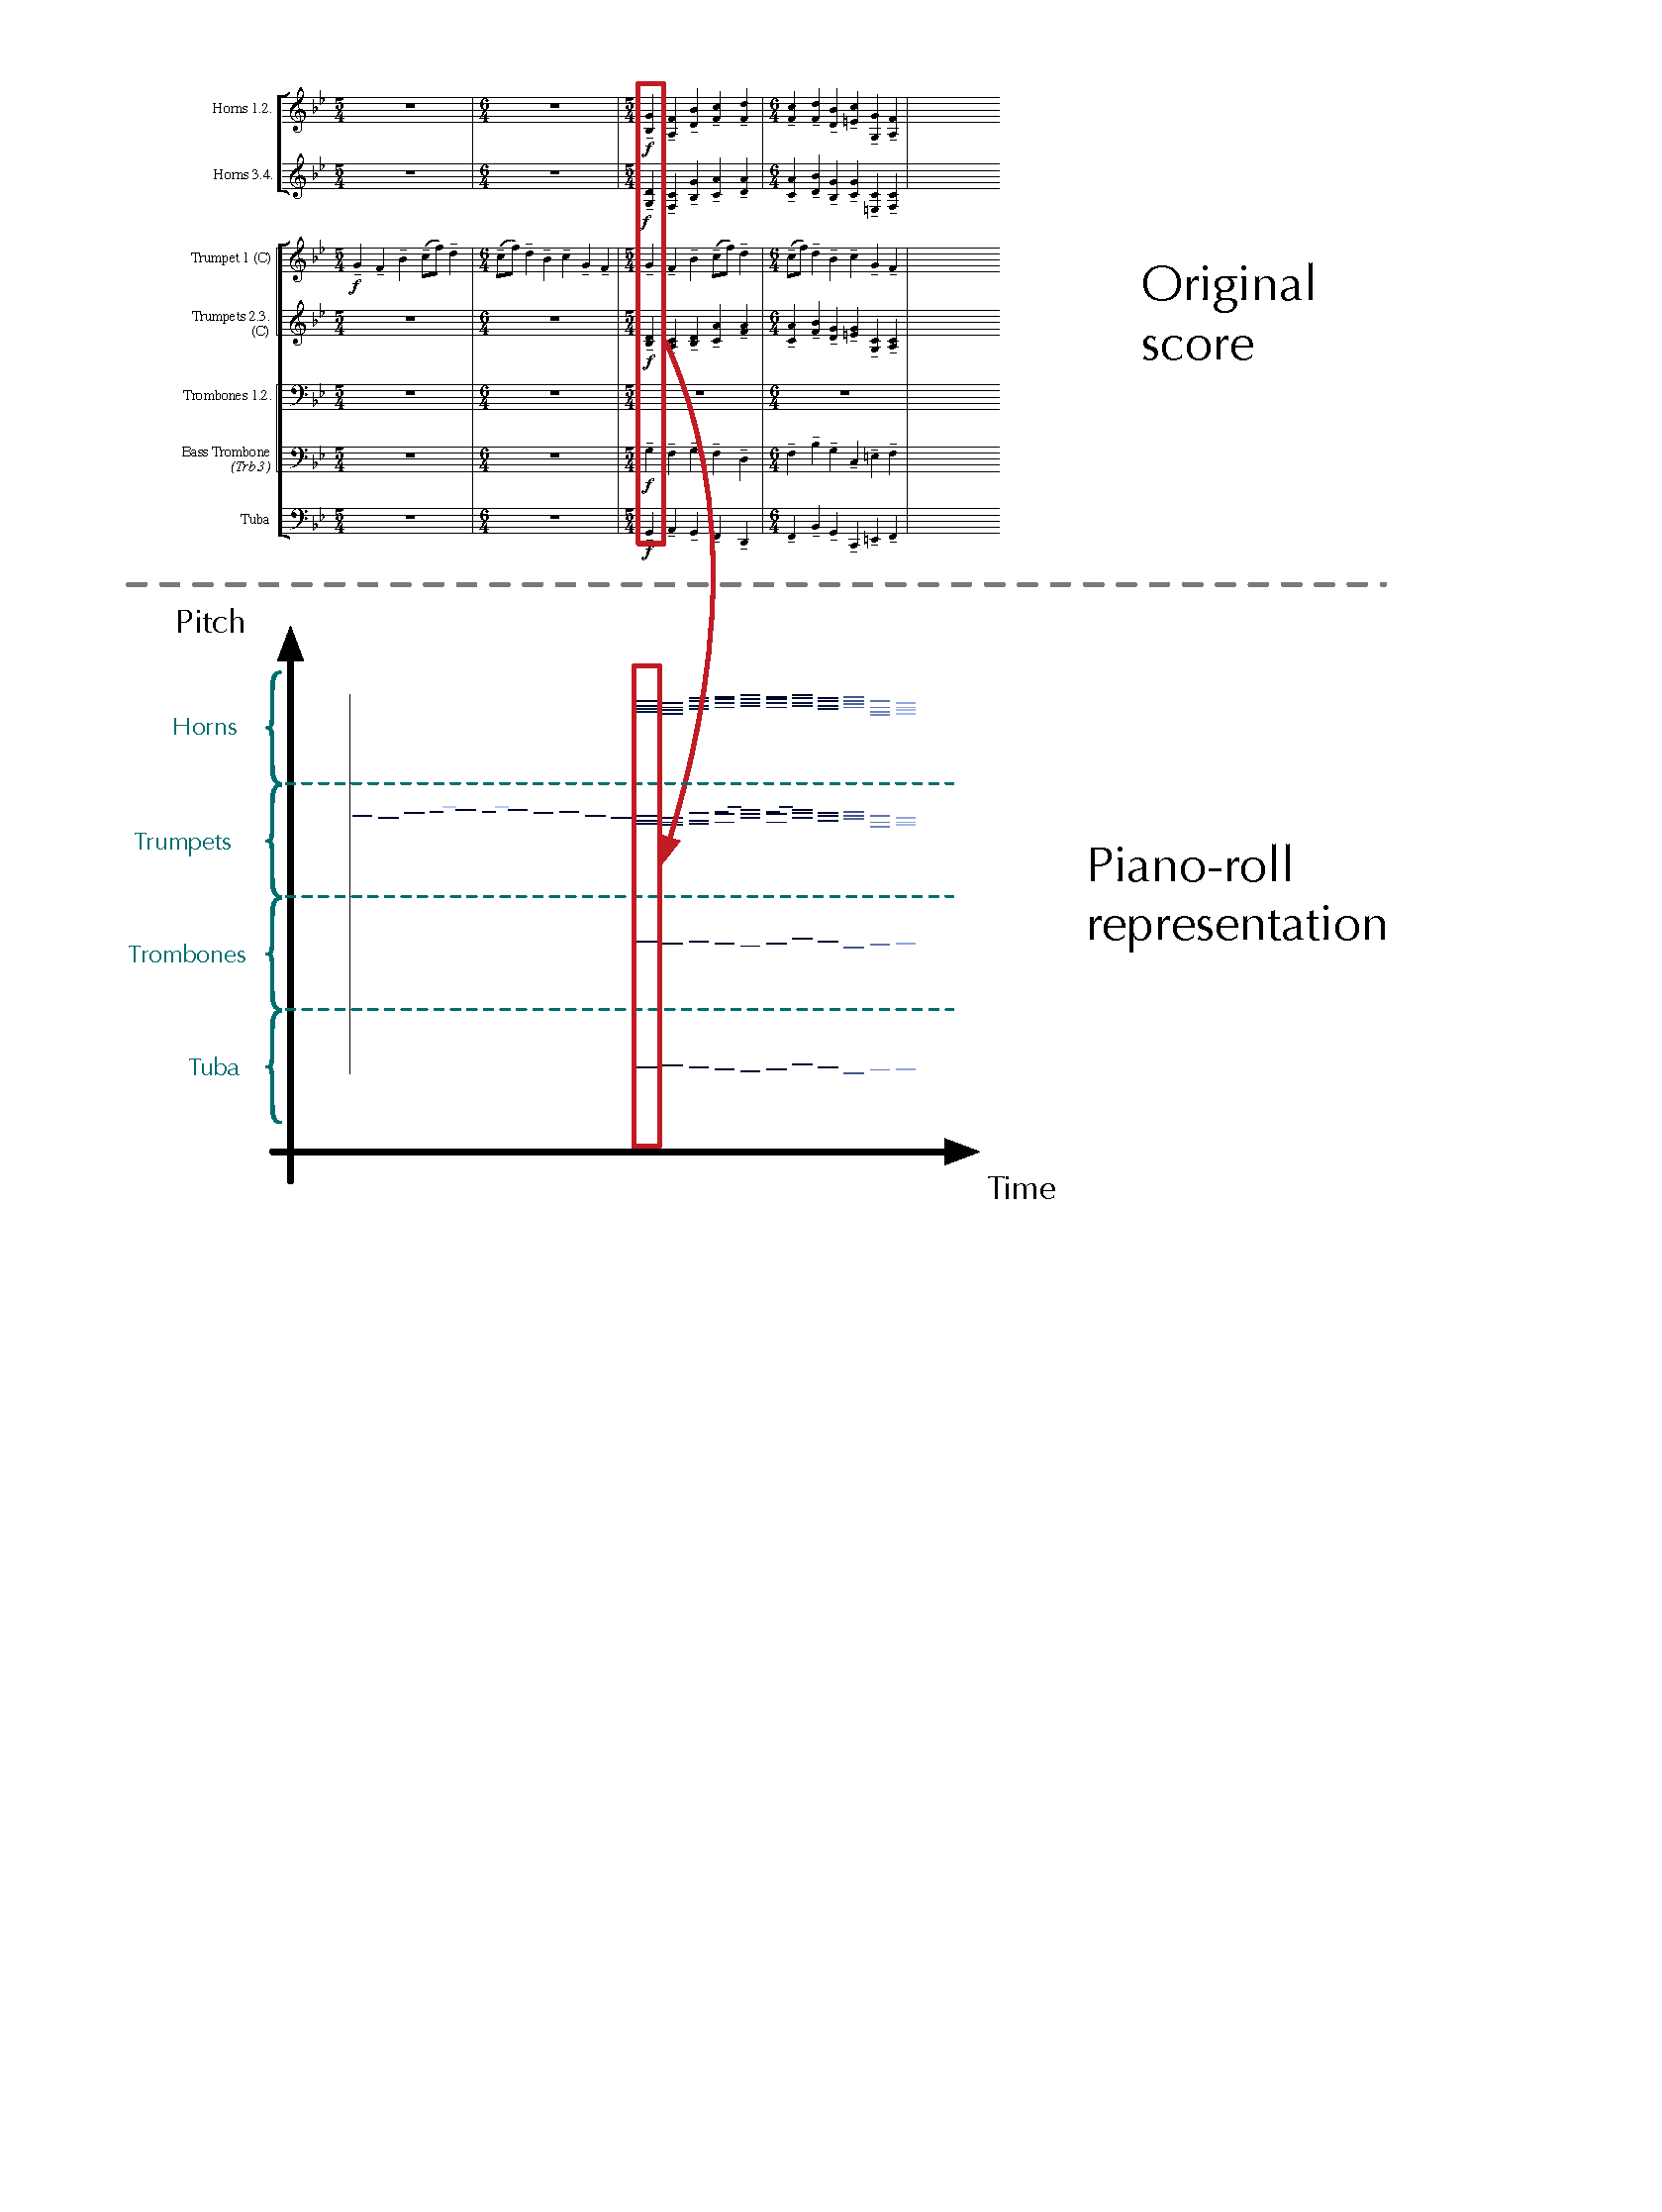
\includegraphics[scale=0.37]{Data_representation/from_score_to_pianoroll}
\caption{From the score of an orchestral piece, a convenient representation for computer processing named \textit{piano-roll} is extracted. A piano-roll $pr$ is a matrix whose rows represent pitches and columns represent a time frame depending on the time quantization. A pitch $p$ at time $t$ played with an intensity $i$ is represented by $pr(p,t) = i$, $0$ being a note off. This definition is extended to an orchestra by simply concatenating the \textit{piano-rolls} of every instruments along the pitch dimension.}
\label{fig:piano-roll}
\end{figure}

\subsubsection{Temporal granularities}
 \begin{figure}
\centering
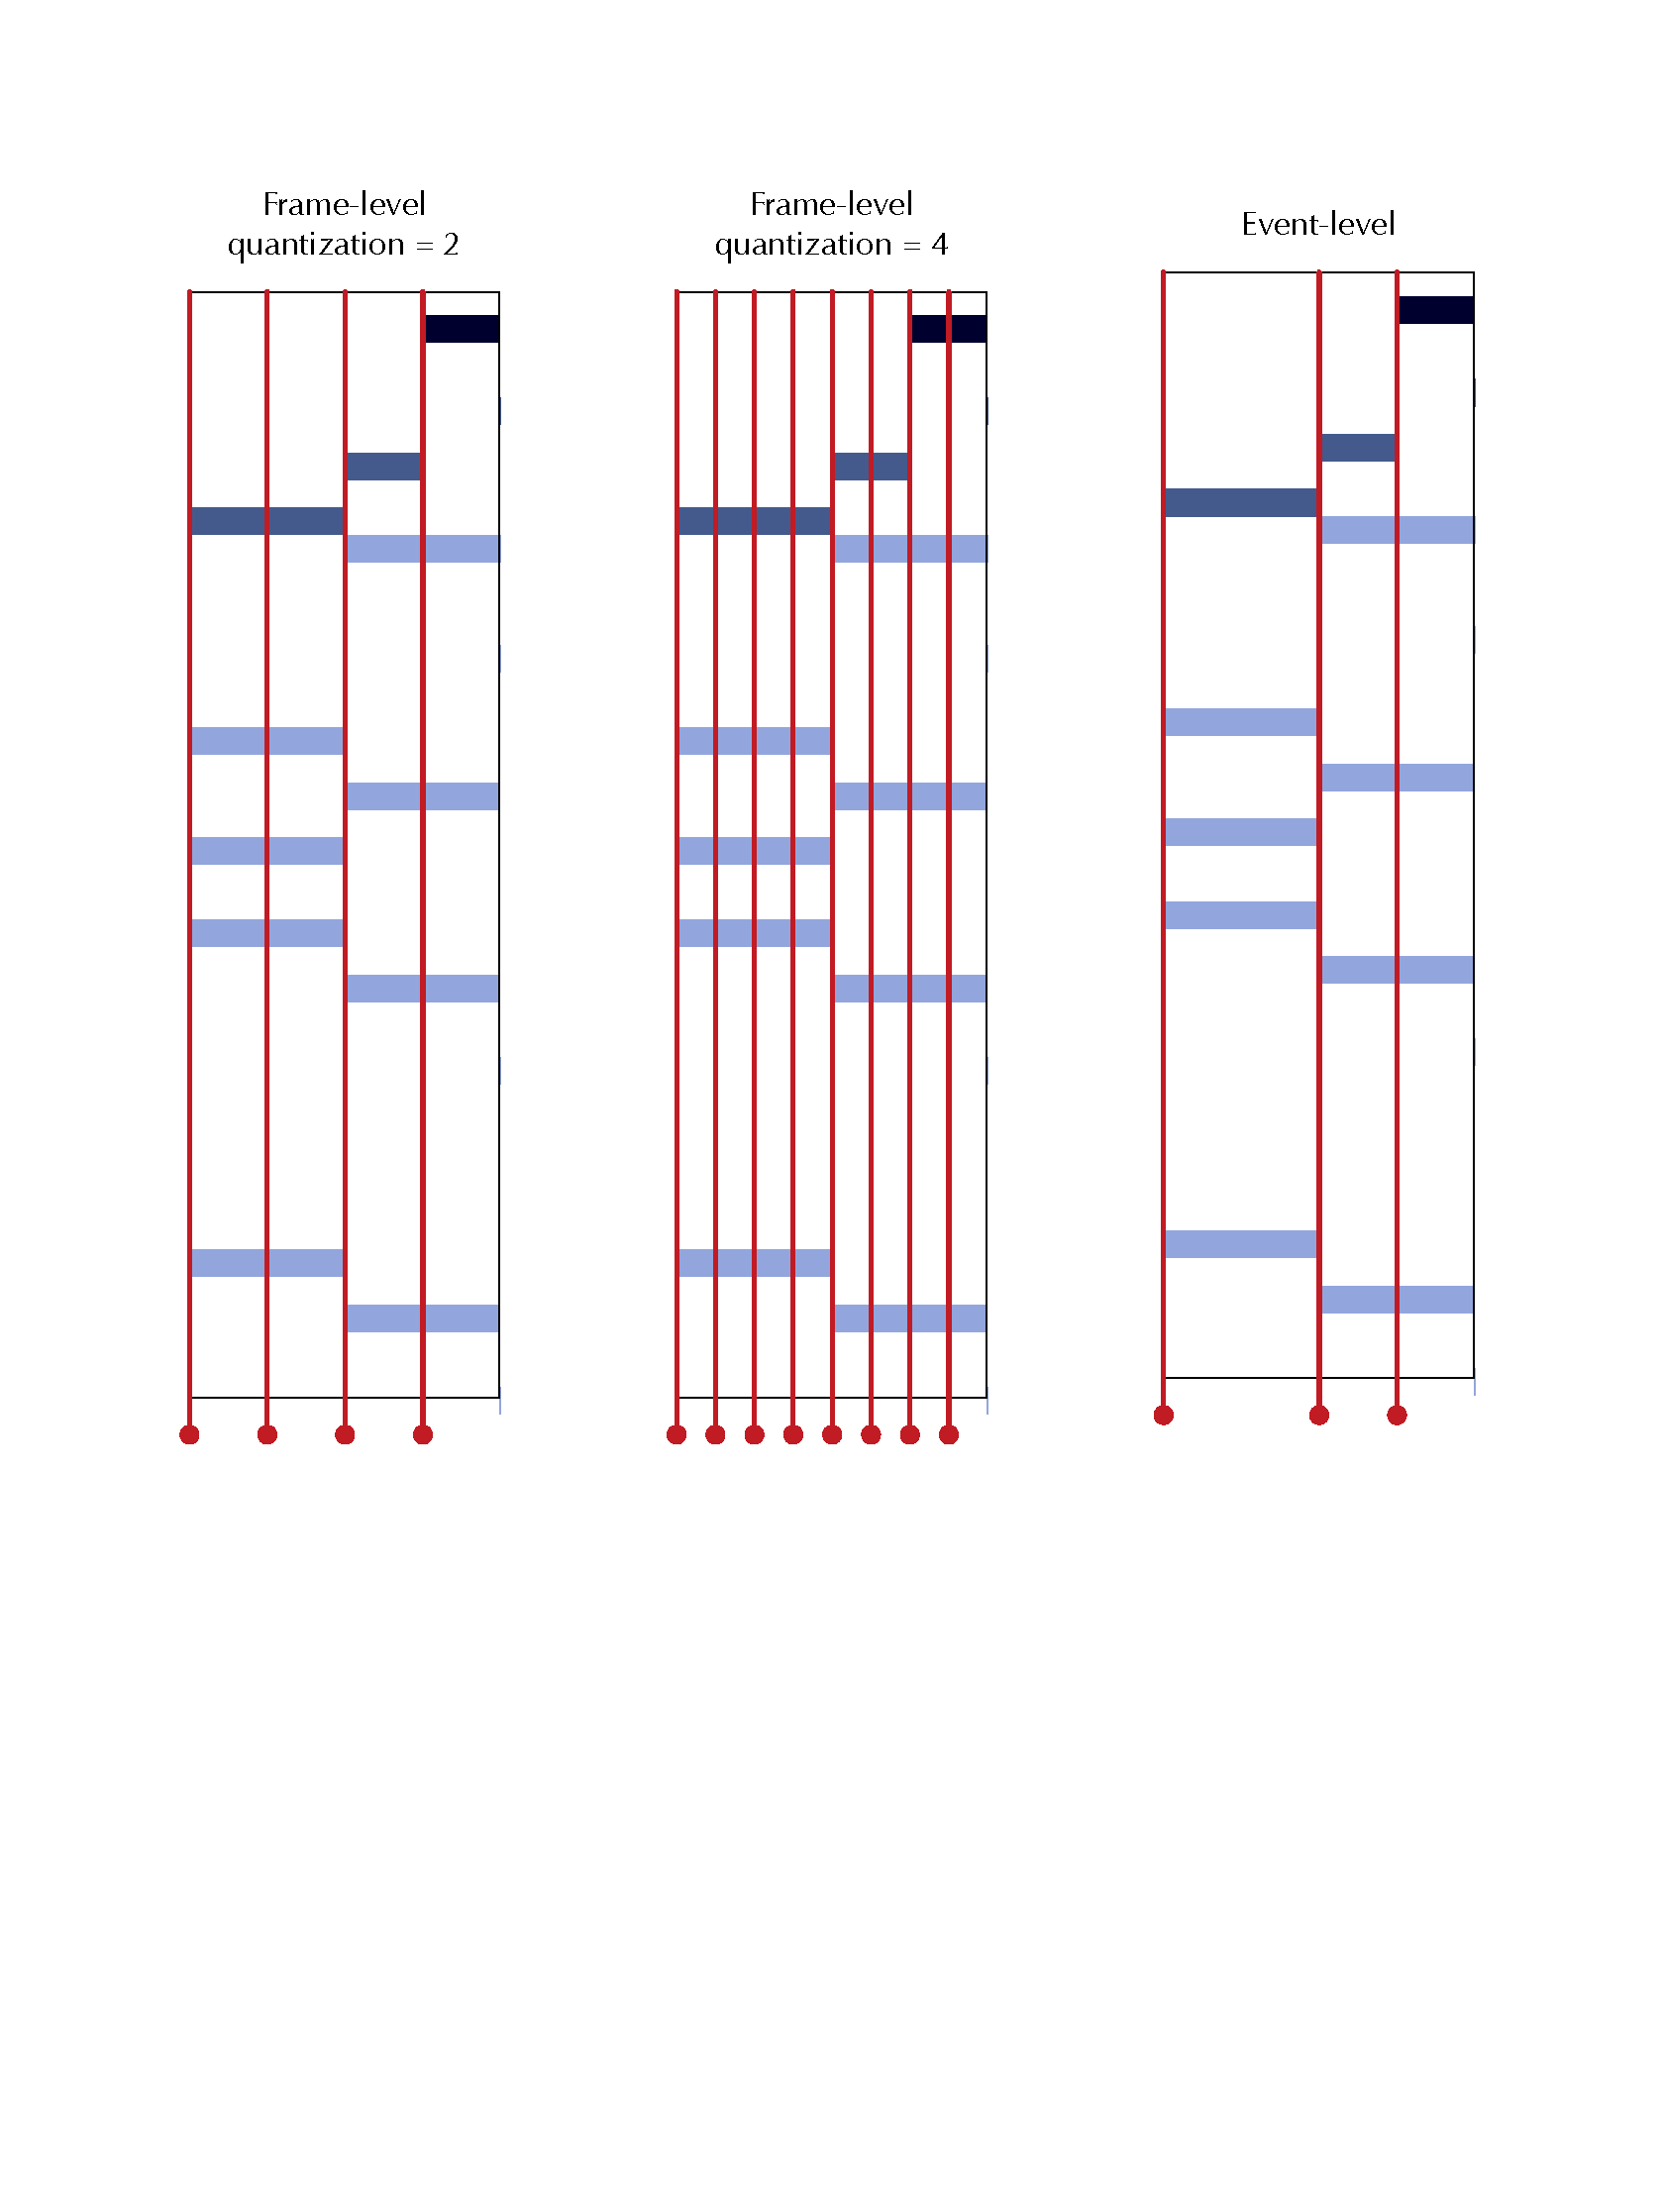
\includegraphics[scale=0.4]{Data_representation/frame_vs_event}
\caption{Frame level and event level granularities. By comparing the piano-rolls on the left-hand side and the middle of the figure, we can observe that, in the case of the frame-level granularity, more consecutive frames are identical as the quantization gets finer. We observe on the right-hand piano-roll how those quantization problem can be carried away with the event-level granularity.}
\label{fig:frame_vs_event}
\end{figure}
We defined two \textit{temporal granularities} \ref{fig:frame_vs_event}.
\begin{itemize}
\item The \textit{frame-level granularity} consists in taking each successive frame into consideration in the piano-roll representation. The rhythmic quantization is defined as the number of time frame in the \textit{piano-roll} per quarter note and defines the precision of the frame-level representation.
\item The \textit{event level granularity} consists in conserving only the frames of the piano-roll representation where an event occurs. We define an event as a time $t_{e}$ where $\text{Orch}(t_{e}) \neq \text{Orch}(t_{e} - 1)$.  
% effet : plus de rhythme
Hence, the temporal precision of the event-level representation no longer depends on a quantization parameter and the scores are seen as a succession of events with no rhythmic structure.
% Justification
It can be justified by considering the simplified case where the rhythmic structure of the projected orchestral score is exactly the same as the one of the original piano score. 
This is false in the general case, since a composer can decide to add non-existent event in an orchestration, but it is a reasonable simplification.
\end{itemize}
In the result section, we discuss the impact of the frame-level or event-level granularity over the performances of the different models \ref{sec:results}.

\subsubsection{Dynamics}
Finally, the velocity information is discarded. Indeed, we use binary units which solely indicate if a note is on or off. We know that the velocity information is crucial in order to perform orchestration, since it can impact the number and type of instruments played. However, we believe this first investigation considering solely binaries units can provide a sufficient insight to determine which architectures and mechanisms are the most adapted to the projective orchestration task.

\subsection{Model definition}
We define $O$ and $P$ as the sequences of column vectors of the \textit{piano-rolls}.
\subsubsection{RBM}
In the case of projective orchestration, the visible units are defined as the concatenation of the past and present orchestra vector and the present piano vector
\begin{equation}
\label{eq:visible_rbm}
\bm{v} = \left[P(t),O(t-N),...,O(t)\right]
\end{equation}

% = negative particule of the CD !!
Generating values from a \textit{RBM} consists in sampling from the visible distribution $p(v)$. However, there is no way to sample directly from this distribution, and computing the probability of each visible unit configuration is computationally intractable.
However, the negative sample of a Gibbs chain is sampled from a approximation of the model distribution, at the condition that the number of steps is sufficiently large. We discuss in the result section \ref{sec:results} how the number of Gibbs sampling step can impact the performances of the model.

% Pbm, in the case of RBM simple generate piano + orchestra -> generation through inpainting
However, in the case of projective orchestration, the vectors $P(t)$ and $[O(t-N), ..., O(t-1)]$ are known, and only the vector $O(t)$ has to be generated. 
Thus, it is possible to infer the negative samples of the CD algorithm while clamping $O(t-N), ..., O(t-1)$ and $P(t)$ to their known values. This technique is known as \textit{inpainting} \cite{Fischer2012}.

Note, however, that extensive efforts are made during the training phase to infer values that are finally clamped during the generation phase. Conditional models offer a way to separate the context (past orchestra and present piano) from the data we actually want to generate (present orchestra).

 \begin{figure*}
 	\begin{centering}
 		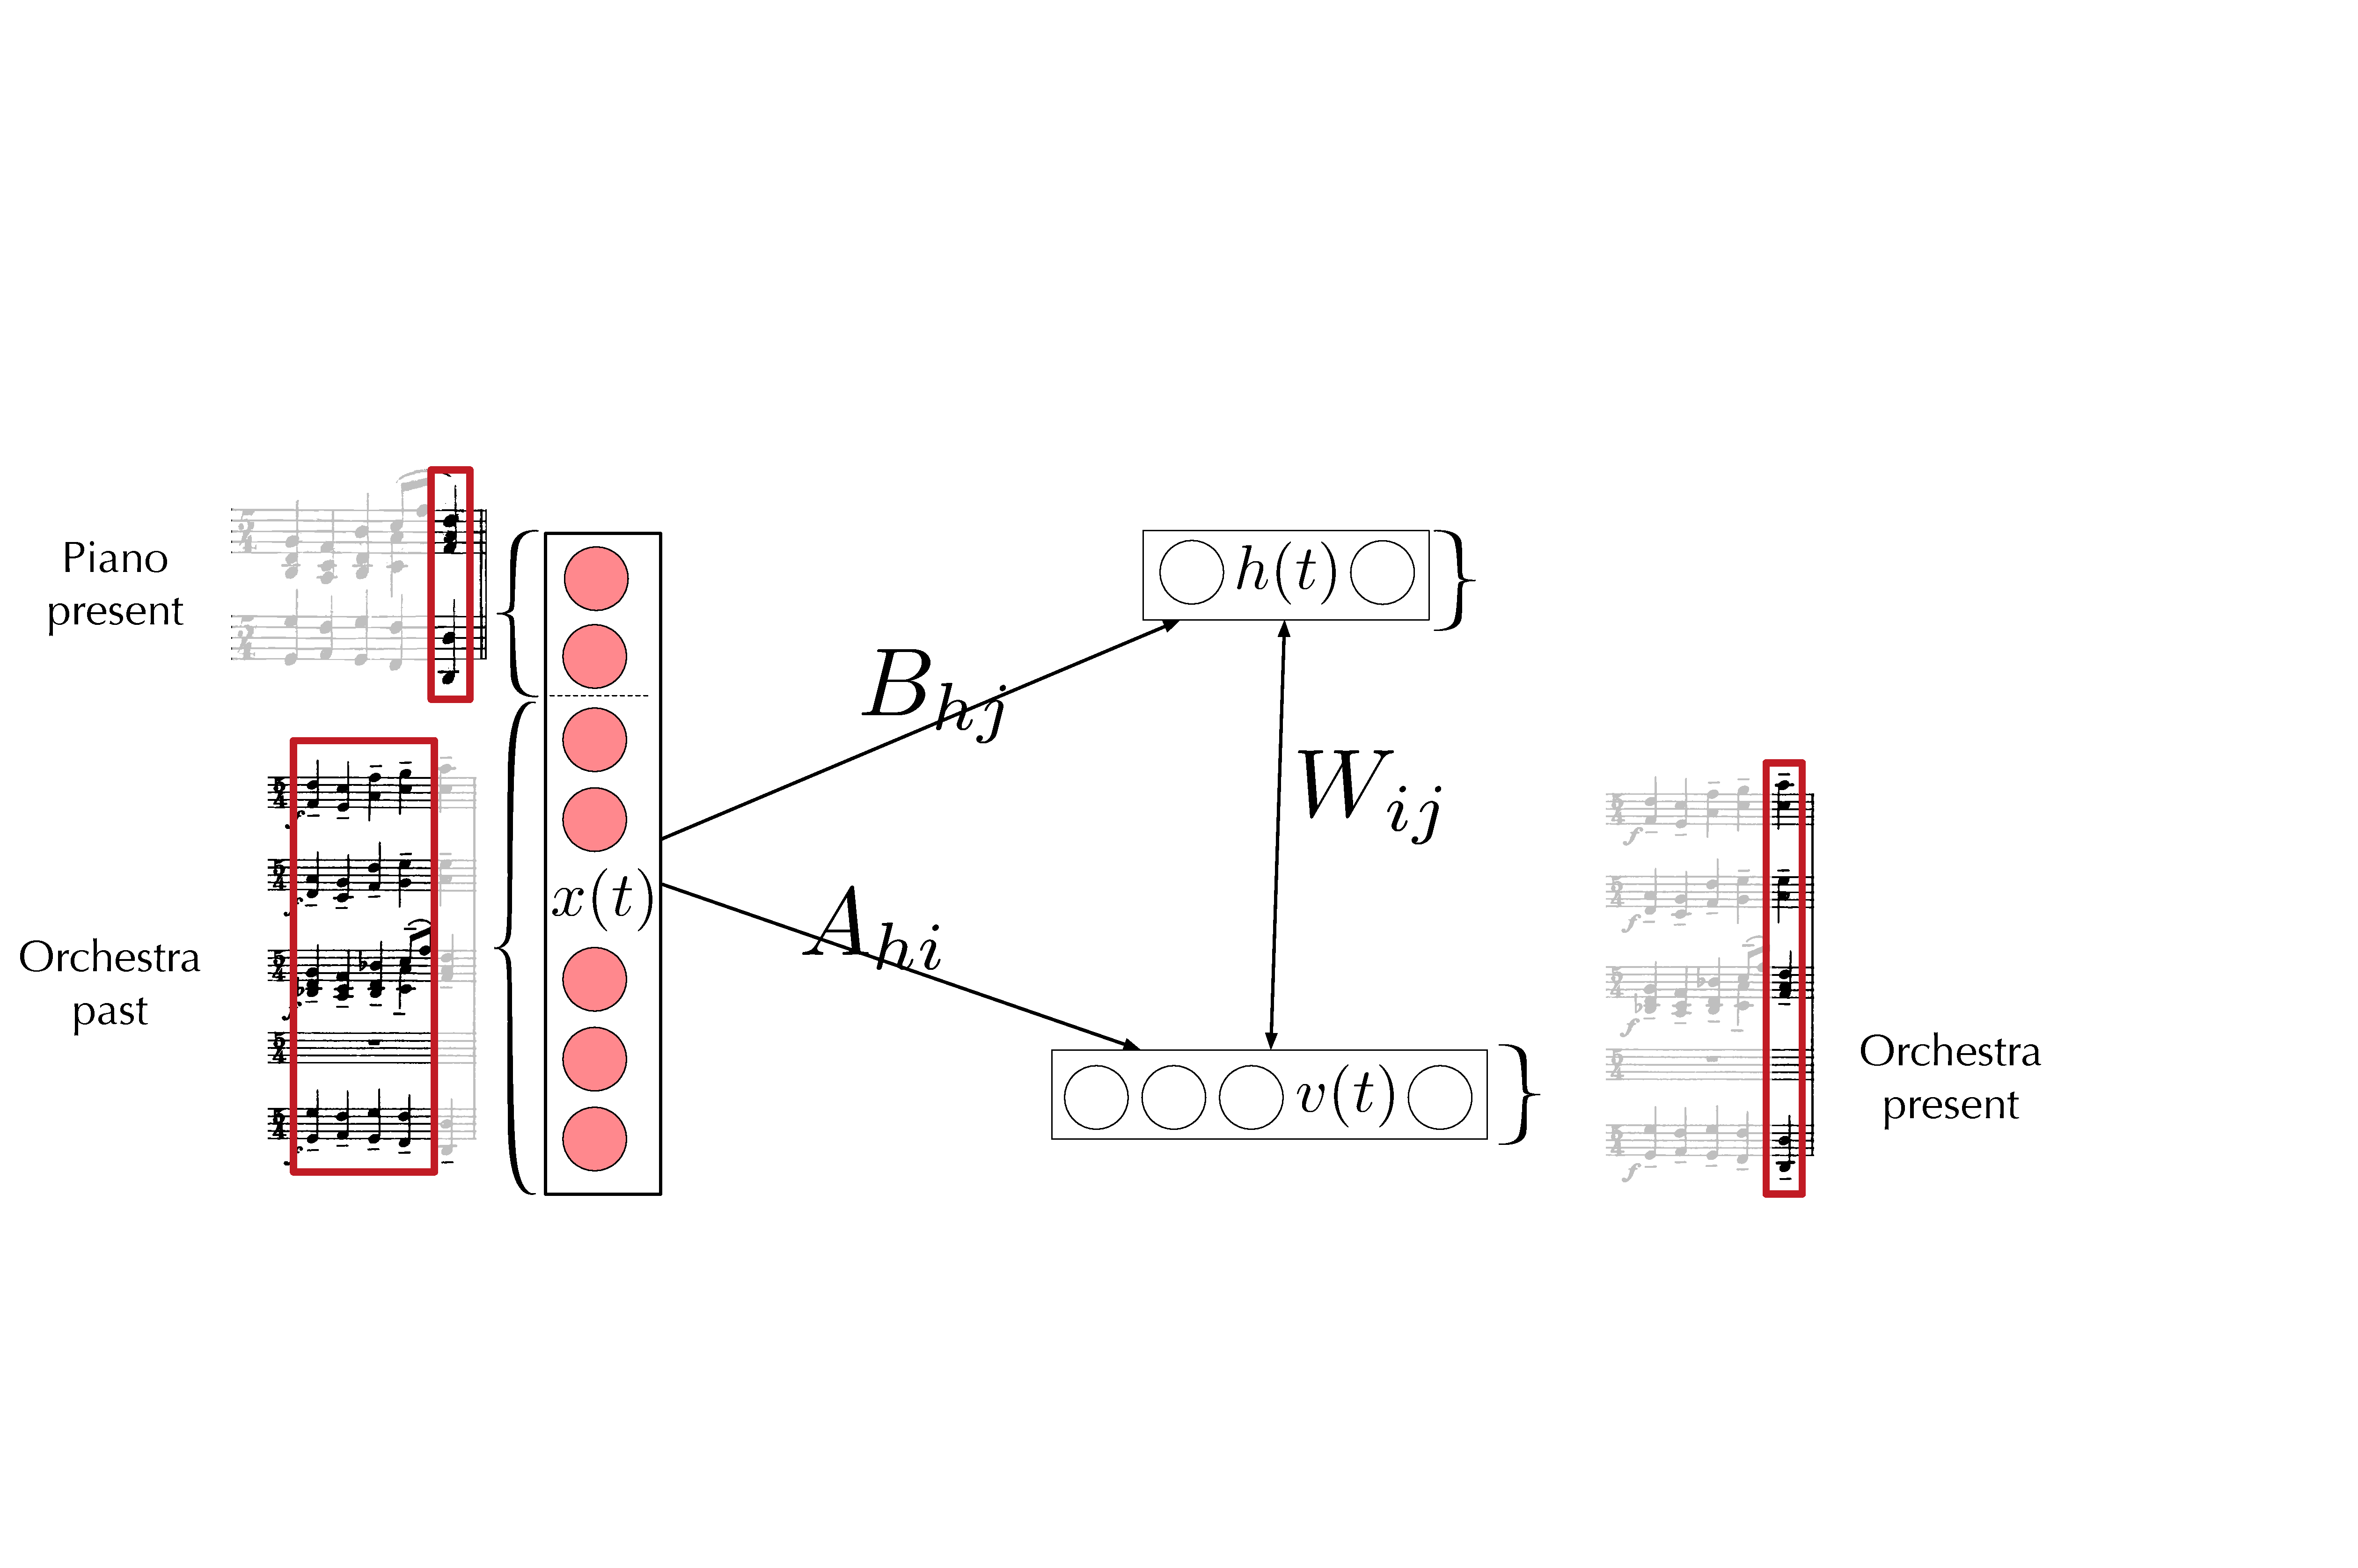
\includegraphics[scale=0.2]{Models/lop_models}
 		\par\end{centering}
 	\caption{Conditional Restricted Boltzmann Machine in the context of projective orchestration. The visible units $\bm{v}$ represent the present orchestral frame $O(t)$. The context units $\bm{x}$ represents the concatenation of the past orchestral and present piano frames $[P(t), O(t-N), ..., O(t-1)]$}.
During the generation phase, after training the model, the context units are clamped to the known values of these vectors.
 	\label{fig:lop_models}
 \end{figure*}
\subsubsection{cRBM and FGcRBM}
% Application orchestration
In the case of projective orchestration, the \textit{cRBM} units' are defined as
\begin{align*}
\bm{v} &= O(t) \\
\bm{x} &= \left[P(t), O(t-N), ..., O(t-1)\right]
\end{align*}
and the \textit{FGcRBM} units' as
 \begin{align*}
 \bm{v} &= O(t) \\
 \bm{x} &= \left[O(t-N), ..., O(t-1)\right]\\
 \bm{z} &= \left[P(t)\right]
 \end{align*}
 
Since the visible units of the \textit{cRBM} and \textit{FGcRBM} models directly represent the present orchestral frame, generating from these two models is straightforward : 
\begin{itemize}
	\item the context units (and latent units in the case of the \textit{FGcRBM}) are set to their known values
 	\item the visible units are randomly initialize with a uniform distribution on the segment $[0,1]$
 	\item several steps of Gibbs sampling are performed
 	\item the visible units sample obtained at the end the Gibbs chain is the vector $\hat{O}(t)$ generated by the model
 \end{itemize}
 Even if visible units represent binaries values, real values can be used during alternate Gibbs sampling \cite{hinton2010practical}. We observed that initializing visible units with a uniform distribution on $[0,1]$ rather than with a Bernouilli distribution leads to slightly better generations. Our guess is that it avoid the model to be stuck in a certain configuration at an early step of the alternate Gibbs sampling process.

\subsection{Evaluation framework}
We introduce an \textit{event-level orchestral inference} task to evaluate our models. To our best knowledge, this is the first attempt to define a quantitative evaluation framework for automatic projective orchestration.

% Split train/valid/test
In order to evaluate the models, the data used to train and those used to assess the performances must be different \cite{bishop2006pattern}. Hence, the dataset is usually split between train, validate and test sets. The repartition we used is indicated in text files at the same location as the database. 

Predictive symbolic music tasks are usually evaluated through a \textit{frame-level} accuracy measure where each time frame of the piano-roll is considered as a separate data example \cite{DBLP:journals/corr/YaoCVDD15,boulanger2012modeling,lavrenko2003polyphonic}.
We propose to work in an \textit{event-level} framework \ref{sec:data_representation}. The reason why we do not rely on a \textit{frame-level} evaluation is that a model which simply repeats the previous frame gradually becomes the best model as the quantization gets finer.

\subsection{Measure}
An objective criterion of the performances of the models is necessary to provide an evaluation. 
The best way for evaluating generative models is to compute the likelihood of the test set (see equation \ref{eq:likelihood}). However, we have seen that this quantity is intractable in all \textit{RBM}, \textit{cRBM} and \textit{FGcRBM} models. 
An alternative criterion commonly used in the music generation field is the accuracy measure \cite{DBLP:journals/corr/YaoCVDD15,boulanger2012modeling,lavrenko2003polyphonic}. For each \textit{event} $t_{e}$ (see previous section), the visible units of the model are sampled with its context (and features for the FGcRBM) units set to $Orch(t_{e}-1),... Orch(t_{e}-N)$ and $Piano(t_{e})$ from the test dataset. This sampled prediction $\text{Pred}(t_{e})$ is then compared to the ground-truth vector $\text{Orch}(t_{e})$ from the test dataset via the accuracy measure
\begin{equation}
\text{Accuracy}  = \frac{TP(t)}{TP(t) + FP(t) + FN(t)}
\label{eq:accuracy}
\end{equation}
where $TP(t)$ (true positives) is the number of notes correctly predicted (note played in the prediction and ground-truth). $FP(t)$ (false positive) is the number of notes predicted which are not in the original sequence (note played in the prediction, but not in ground-truth). $FN(t)$ (false negative) is the number on unreported notes (note absent in prediction, but played in ground-truth). 
Instead of binary values, activation probabilities are used for the predicted samples in order to avoid sampling noise.

\subsection{Results}
\label{sec:results}
Five models are evaluated on the orchestral inference task. The first model is a random generation of the orchestral frames from a Bernoulli distribution of parameter $0.5$. The second model predicts an orchestral frame at time $t$ by repeating the frame at time $t-1$. Those two naive models constitute a first baseline against which we compare the \textit{RBM}, \textit{cRBM} and \textit{FGcRBM} models.

% Hyper-parameters
For the three last models, 50 random configurations have been evaluated over the hyper-parameter space and we retained the best score. 

Examples of produced orchestration, implementations and details about the hyper-parameters search can be found at this address \url{https://qsdfo.github.io/LOP/}.

\begin{table}[h]
	\centering
	\begin{tabular}{c c c}
		\hline
		\thead{Model} & \thead{Frame-level\\ accuracy} & \thead{Event-level\\ accuracy} \\
		\hline
		Random & ? & ?\\ 
		Repeat & ? & ?\\
		\hline \hline
		RBM & ? & 1.39\\ 
		cRBM & ? & 27.67\\ 
		FGcRBM & ? & 25.80\\ 
	\end{tabular}
	\caption{Event-level and frame-level (with quantization 4) accuracy for the orchestral inference task.}
	\label{tab:result_event_level}
\end{table}
The results are summed up in table \ref{tab:result_event_level}.

% Frame VS event
The effect of the quantization can be observed, as the repeat model outperforms all the other models as the quantization gets finer.

% Context = good
For the event-level granularity, the two conditional architectures largely outperform the random, repeat and RBM models, which justify the introduction of context units.
% Factor = not that good
However the \textit{FGcRBM} has slightly worst performances than the \textit{cRBM}.
Hence, the introduction of three ways interactions has not proved to be useful in the case of projective orchestration.

\subsection{Qualitative analysis}
To gain better insight into these results, orchestration can be observed for each model on the website \url{https://qsdfo.github.io/LOP/}.
% Corrupted
Since there is no distinction between the piano and orchestra frames in context units of the cRBM, we were afraid at some point that only one of the two information were actually used by the model. To estimate the importance of the past orchestral and the present piano frames on the orchestration, we generated \textit{corrupted} sequences, where either the piano, either the orchestra is clamped to zero. We observed that the results dramatically decrease when one of the two information is missing.

\subsection{Discussion : evaluating a generative model ?}
It is important to state that we do not consider this predictive measure as as reliable measure of the creative performance of a model. Indeed, predicting and creating are two fairly different things. 
Hence, the predictive evaluation framework we have built does not assess the generative ability of a model, but is rather used as a selection criterion among different models.

\section{Live Orchestral Piano (LOP)}
We introduce in this section the \emph{Live Orchestral Piano} (LOP)
application, which is the first software able to provide a way to
compose music with a full classical orchestra in real-time by simply
playing on a MIDI piano. The goal of this framework is to rely on
the knowledge learned by the model introduced in the previous sections
in order to perform the projection from a piano melody to the orchestra.

\subsection{Workflow}
The software is implemented on a client/server paradigm. This choice
allows to separate the orchestral computation part from the interface
and sound rendering engine. That way, multiple interfaces can easily
be implemented. It should also be noted that separating the computing
and rendering on different computers, can allow to use high-quality
and CPU-intensive orchestral rendering plugins. This can allow a more
realistic orchestral rendering with heavy amounts of computation performed
while ensuring the real-time constraint on the overall system (preventing
degradation of the computing part). The complete implementation workflow
is presented in Figure~\ref{fig:Live-orchestral-piano}.

\begin{figure*}
\begin{centering}
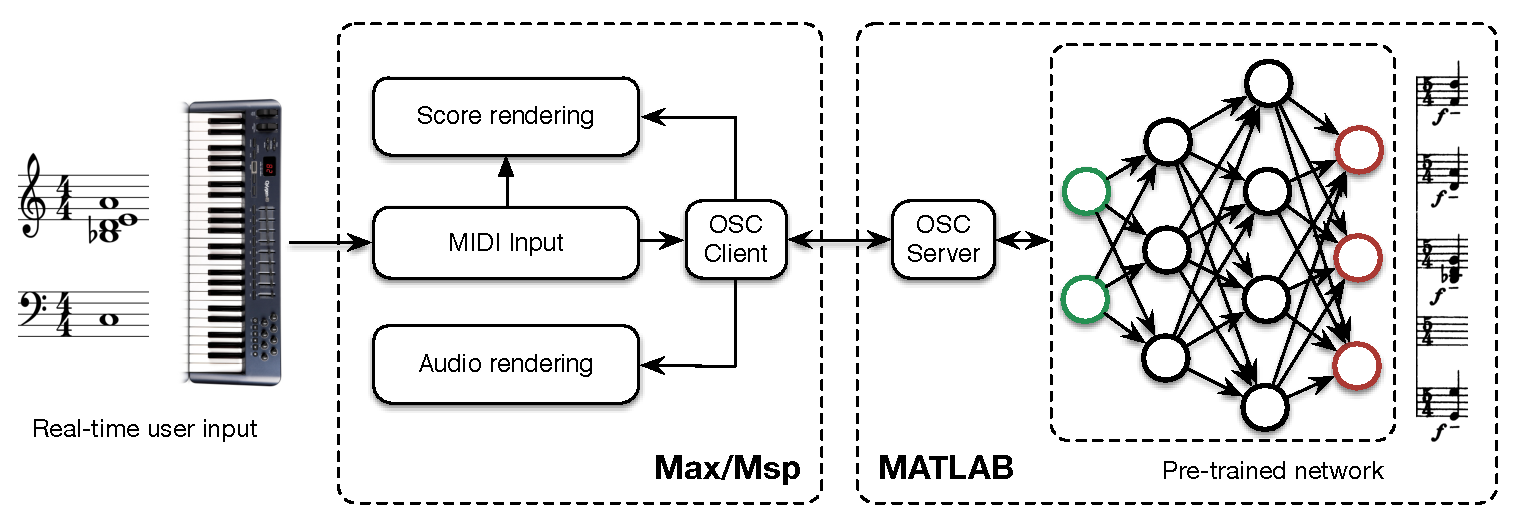
\includegraphics[scale=0.55]{workflow}
\par\end{centering}
\caption{\label{fig:Live-orchestral-piano}Live orchestral piano (L.O.P) implementation
workflow. The user inputs a melody which is transcribed into a score
and send via OSC from the Max/Msp client. Then, the MATLAB server
uses this vector of notes and process it following the aforementioned
techniques in order to obtain the orchestration. This information
is then sent back to Max/Msp which performs the real-time audio rendering }
\end{figure*}

As we can see, the user can input a melody (single notes or chords)
through a MIDI keyboard, which is retrieved inside the Max/Msp interface.
The interface transmits this symbolic information (as a variable-length
vector of active notes) via OSC to the MATLAB server. The interface
performs a real-time transcription of the piano score to the screen
in parallel. The server uses this vector of events to produce an 88
vector of binary input note activations (as defined in the sub-section \textit{Data representation}).
This vector is then processed by using the orchestration algorithms
presented in sub-section \textit{Model definition} in order to obtain a projection
of a specific symbolic piano melody to the full orchestra (an operation
defined as \emph{projective orchestration}). The resulting orchestration
is then sent back to the client interface which performs both the
real-time audio rendering and score transcription. 

\subsection{Interface}
The interface has been developed in Max/Msp, to facilitate both the
score and audio rendering aspects in a real-time environment. The
score rendering is handled by the \emph{Bach} library environment. 
This interface provides a way to easily switch between different orchestration models, while controling other
meta-parameters of the sampling. For instance the \emph{cutoff probability
}gives a direct access to the density of the generated orchestration
(in terms of number of played instruments). Indeed, a low cutoff probability
implies that most activation of notes will be taken into account in
the playback, while a high cutoff will produce more sparse orchestration.

\section{Conclusion and future works}
% Orchestral inf problem
We have introduced a system for real-time projective orchestration of a midi piano input. In order to select the most adapted model, we have proposed an evaluation framework called orchestral inference which rely on an orchestral inference task. We have assessed the performance of the cRBM and FGcRBM, and observed the better performances of the cRBM model.

% Interesting and highly benefit problem
The general objective of building a generative model for time series is one of the most prominent topic for the machine learning field. Orchestral inference sets a slightly more specific framework where the generated time series is conditioned by an other observed time series (the piano score). Besides, being able to grasp the long range dependencies structuring music appears as a challenging and worthwhile task.

% Increase DB
%The high dimensionality of the data and their sparsity are a major obstacle for learning algorithms.
%A first remark is that a larger database would be required to train any model sufficiently complex to properly represent the underlying distribution of a projective orchestration.
%It is important to build a reference database of piano scores and their orchestration by acknowledge composers, with all instrument name indicated and velocity for the notes

% More models
% Condi = good 
% Mix with temporal ?
The conditional models have proven to be effective in the orchestral inference evaluation framework we defined. The observations of the orchestration generated by the models tend to confirm these performance scores, and is a confirmation of the soundness of the framework.
However, we believe that the performances can be further improved by mixing conditional models and recurrent models such (Recurrent Neural Networks).

% Velocities
The most crucial improvement to our system is to include the dynamic of the notes.
Indeed, many orchestral effects are justified by intensity variations in the original piano scores. 
Hence, by using binaries units, an essential  information is discarded.
% Find distrib representations
Finally, the sparse representation of the data suggests that a more compact distributed representation might be found. Lowering the dimensionality of the data would greatly improve the efficiency of the learning procedure. For instance, methods close to the word-embedding techniques used in natural language processing might be useful \cite{kiros2015skip}.

\section{Acknowledgements}
This work has been supported by the \textit{NVIDIA GPU Grant} program.
The authors would like to thank Denys Bouliane for kindly providing the orchestral database.

%%%%%%%%%%%%%%%%%%%%%%%%%%%%%%%%%%%%%%%%%%%%%%%%%%%%%%%%%%%%%%%%%%%%%%%%%%%%%
%bibliography here
\bibliography{../Biblio/biblio}

\end{document}
